\section{Introduction}

\begin{figure}[H]
  \centering
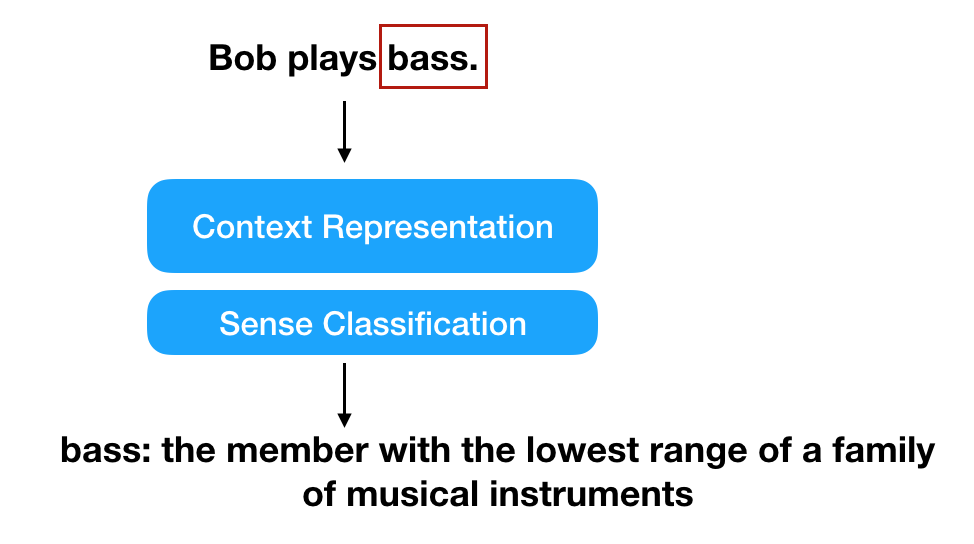
\includegraphics[width=0.5\textwidth]{graphs/overview.png}
\caption{system overview}
\end{figure}

We rely on Google to retrive information. The typical way we interact with
search engines is typing in search key words using natural languages. However
English words have different meanings in different contexts. A major challenge
to precisely retrive the desired information is for search engine to understand
the meaning of key words in a given context.

To solve this problem, we propose to build a word sense disambiguate system that
takes an English word and a sentence where it appears as input, and predicts the
sense of such word with regard to the given context. 

A pratical usage of our system, would be for the search engine to substitute the
key words with paraphases of the same predicted sense, thus it can retrive a
more complete set of results for a given user query.
